\documentclass{article}

\usepackage{color}
\usepackage[margin=1in]{geometry}
\usepackage{graphicx}
\usepackage{hyperref}
\usepackage{listings}

\definecolor{gray}{rgb}{0.5, 0.5, 0.5}
\definecolor{darkgreen}{rgb}{0, 0.6, 0}

\begin{document}
    \raggedright
    Homework 3 \break
    Christopher Seagraves
% % % % % % % % % % % % % % % % % % % % % % % % % % % % % % % % % % % % % % % % 

    \section*{Problem 1}
        \begin{minipage}{\linewidth}
            \raggedright
            I'm sorry for being lazy, but hopefully doing 6 or so nodes is enough to prove I could have continued...
            \begin{center}
                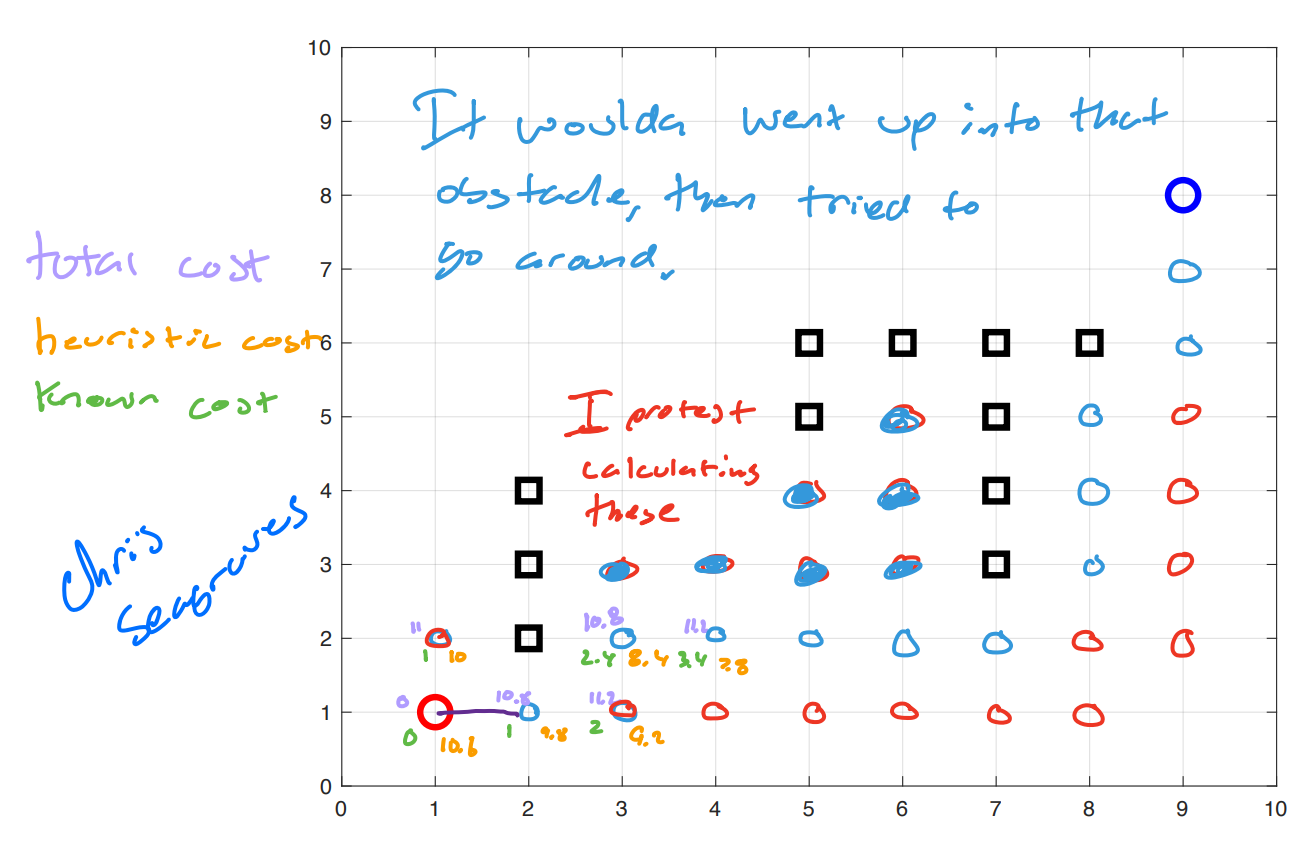
\includegraphics[width=\linewidth]{HW3P1 A Star by hand.png}
            \end{center}
        \end{minipage}
% % % % % % % % % % % % % % % % % % % % % % % % % % % % % % % % % % % % % % % %
    
        \section*{Problem 2}
            \begin{minipage}{\linewidth}
                \raggedright
                ./main.py \break
                \url{https://github.com/nosv1/seagraves_unmanned_systems/blob/main/HW3/main.py} \break
                ./AStar.py \break
                \url{https://github.com/nosv1/seagraves_unmanned_systems/blob/main/HW3/AStar.py}
            \end{minipage}
% % % % % % % % % % % % % % % % % % % % % % % % % % % % % % % % % % % % % % % % 

        \section*{Problem 3}
            \begin{minipage}{\linewidth}
                \raggedright
                ./main.py \break
                \url{https://github.com/nosv1/seagraves_unmanned_systems/blob/main/HW2/main.py} \break
                ./Dijkstra.py \break
                \url{https://github.com/nosv1/seagraves_unmanned_systems/blob/main/HW2/Dijkstra.py}
            \end{minipage}
% % % % % % % % % % % % % % % % % % % % % % % % % % % % % % % % % % % % % % % % 

\end{document}